
%=+=+=+=+=+=+=+=+=+=+=+=+=+=+=+=+=+=+=+=+=+=+=+=+=+=+=+=+=+=+=+=+=+=+=+=+=+=+=+=
%             _             _
%            | |           | |
%  _ __ ___  | |__    ___  | | ___   ___   _ __       ___   ___   _ __ ___ 
% | '_ ` _ \ | '_ \  / _ \ | |/ __| / _ \ | '_ \     / __| / _ \ | '_ ` _ \ 
% | | | | | || | | || (_) || |\__ \| (_) || | | | _ | (__ | (_) || | | | | | 
% |_| |_| |_||_| |_| \___/ |_||___/ \___/ |_| |_|(_) \___| \___/ |_| |_| |_| 
%
% Author: Mark H. Olson
% Website: https://mholson.com
% Github: https://github.com/mholson
%
% Created: 2015-07-31
%
% Enter Text here
%=+=+=+=+=+=+=+=+=+=+=+=+=+=+=+=+=+=+=+=+=+=+=+=+=+=+=+=+=+=+=+=+=+=+=+=+=+=+=+=

%=-=-=-=-=-=-=-=-=-=-=-=-=-=-=-=-=-=-=-=-=-=-=-=-=-=-=-=-=-=-=-=-=-=-=-=-=-=-=-=
% PREAMBLE :: main.tex 
%=-=-=-=-=-=-=-=-=-=-=-=-=-=-=-=-=-=-=-=-=-=-=-=-=-=-=-=-=-=-=-=-=-=-=-=-=-=-=-=
%
% > > >	The following beamer class options are available
%?		aspectratio			= 169
%?		sectionpages
%
% > > > The following sthlmnord package options are available
%?		mode				= dark (default)
%?							= light
%=-=-=-=-=-=-=-=-=-=-=-=-=-=-=-=-=-=-=-=-=-=-=-=-=-=-=-=-=-=-=-=-=-=-=-=-=-=-=-=

\documentclass[aspectratio=169, sectionpages]{beamer}
%\usetheme[mode=light]{sthlmnord}
\usetheme{sthlmnord}

% > > > CTAN Packages
%		the subfiles package is being used to compile individual slides
%		using the main tex file.  Individual slides can then be included
%		into multiple slide decks.
\usepackage{subfiles}

% > > > Custom Packages
\usepackage{mhomacros}
\usepackage{mhotables}



% > > > Generate some Lorem Ipsum placeholder text.
\usepackage{lipsum}

% > > > verbatim 
\usepackage{verbatim}

% > > >Bibliography
\usepackage{cleveref}
\usepackage[backend=biber,style=numeric]{biblatex}
\addbibresource{mhoRef.bib}

% > > >	Image File Paths
% 		Here you can add one or more paths to where your images are being
%		stored.  This will allow you to include only the image file 
%		name when placing it into your document.
%\graphicspath{{path1},{path2},{path3}}
\graphicspath{{./assets/}} 

\newcommand{\snord}{\cnordTen{sthlm}\cnordEight{NORD}}

% > > > Document Information
\title{sthlmNord Beamer Theme (version 3.1)}
\subtitle{Nord Inspired from Stockholm}
\newcommand{\descMiscI}{Courses Title Goes Here}
\newcommand{\descMiscII}{\currfilebase}
\newcommand{\titleAuthor}{Created by}
\author{mholson.com}
\newcommand{\titleInstitute}{Institute}
\institute{School in Stockholm}
\newcommand{\titleMiscI}{Course}
\newcommand{\titleMiscII}{File}
\date{\today}
\titlegraphic{nordtitlelogolight}

% > > > pdf customizations via hyperref (pkg installed by beamer)
\hypersetup{
%colorlinks=true,
% You might want to disable color links for you final draft 
% AND for colors to work properly where links are included.
colorlinks=false,
linkcolor={nordNine},
citecolor={nordNine},
urlcolor={nordNine}
}

%=-=-=-=-=-=-=-=-=-=-=-=-=-=-=-=-=-=-=-=-=-=-=-=-=-=-=-=-=-=-=-=-=-=-=-=-=-=-=-=
%
%    DOCUMENT BEGINS HERE 
%
%=-=-=-=-=-=-=-=-=-=-=-=-=-=-=-=-=-=-=-=-=-=-=-=-=-=-=-=-=-=-=-=-=-=-=-=-=-=-=-=
\begin{document}

%=-=-=-=-=-=-=-=-=-=-=-=-=-=-=-=-=-=-=-=-=-=-=-=-=-=-=-=-=-=-=-=-=-=-=-=-=-=-=-=
%   TITLE START   -=-=-=-=-=-=-=-=-=-=-=-=-=-=-=-=-=-=-=-=-=-=-=-=-=-=-=-=-=-=-=
\titlepage
%   TITLE END   --==-=-=-=-=-=-=-=-=-=-=-=-=-=-=-=-=-=-=-=-=-=-=-=-=-=-=-=-=-=-=
%=-=-=-=-=-=-=-=-=-=-=-=-=-=-=-=-=-=-=-=-=-=-=-=-=-=-=-=-=-=-=-=-=-=-=-=-=-=-=-=

%=-=-=-=-=-=-=-=-=-=-=-=-=-=-=-=-=-=-=-=-=-=-=-=-=-=-=-=-=-=-=-=-=-=-=-=-=-=-=-=
%   FRAME START   -=-=-=-=-=-=-=-=-=-=-=-=-=-=-=-=-=-=-=-=-=-=-=-=-=-=-=-=-=-=-=
{
	\setbeamertemplate{background canvas}{\begin{tikzpicture}\node[opacity=.8,inner sep=0pt]{\includegraphics
				[width=\paperwidth,keepaspectratio]{nordsegel}};\end{tikzpicture}}
	\begin{frame}[plain]{}
		\addtocounter{framenumber}{-1}
	\end{frame}
}
%   FRAME END   --==-=-=-=-=-=-=-=-=-=-=-=-=-=-=-=-=-=-=-=-=-=-=-=-=-=-=-=-=-=-=
%=-=-=-=-=-=-=-=-=-=-=-=-=-=-=-=-=-=-=-=-=-=-=-=-=-=-=-=-=-=-=-=-=-=-=-=-=-=-=-=


%=-=-=-=-=-=-=-=-=-=-=-=-=-=-=-=-=-=-=-=-=-=-=-=-=-=-=-=-=-=-=-=-=-=-=-=-=-=-=-=
%   TABLE OF CONTENTS START   -=-=-=-=-=-=-=-=-=-=-=-=-=-=-=-=-=-=-=-=-=-=-=-=-=
\begin{frame}
	\frametitle{Table of contents}
	% > > > For longer presentations use \tableofcontents[hideallsubsections] option
	%		It is also possible to manually control the entries of the table of 
	% 		contents by sections.
	%\tableofcontents[sections={1-10}]
	%\framebreak
	%\tableofcontents[sections={11-15}]
	\tableofcontents
\end{frame}
%   TABLE OF CONTENTS END   -=-=-=-=-=-=-=-=-=-=-=-=-=-=-=-=-=-=-=-=-=-=-=-=-=-=
%=-=-=-=-=-=-=-=-=-=-=-=-=-=-=-=-=-=-=-=-=-=-=-=-=-=-=-=-=-=-=-=-=-=-=-=-=-=-=-=



%=-=-=-=-=-=-=-=-=-=-=-=-=-=-=-=-=-=-=-=-=-=-=-=-=-=-=-=-=-=-=-=-=-=-=-=-=-=-=-=
% SECTION 
%=-=-=-=-=-=-=-=-=-=-=-=-=-=-=-=-=-=-=-=-=-=-=-=-=-=-=-=-=-=-=-=-=-=-=-=-=-=-=-=
\section{Background Information}


%=-=-=-=-=-=-=-=-=-=-=-=-=-=-=-=-=-=-=-=-=-=-=-=-=-=-=-=-=-=-=-=-=-=-=-=-=-=-=-=
%   FRAME START   -=-=-=-=-=-=-=-=-=-=-=-=-=-=-=-=-=-=-=-=-=-=-=-=-=-=-=-=-=-=-=
\begin{frame}{Please use Metropolis Theme Instead}

	Thank you for wanting to use sthlmNord version 3.

	\vspace{1em}
	\begin{alertblock}{Warning Label}
		\alert{You really should consider} using the Metropolis
		theme (mTheme) developed \& maintained by Matthias
		Vogelgesang instead. It has been extensively tested, documented and available through CTAN.
	\end{alertblock}
	\begin{center}
		\url{https://github.com/matze/mtheme}
	\end{center}
\end{frame}
%   FRAME END   --==-=-=-=-=-=-=-=-=-=-=-=-=-=-=-=-=-=-=-=-=-=-=-=-=-=-=-=-=-=-=
%=-=-=-=-=-=-=-=-=-=-=-=-=-=-=-=-=-=-=-=-=-=-=-=-=-=-=-=-=-=-=-=-=-=-=-=-=-=-=-=


%=-=-=-=-=-=-=-=-=-=-=-=-=-=-=-=-=-=-=-=-=-=-=-=-=-=-=-=-=-=-=-=-=-=-=-=-=-=-=-=
%   FRAME START   -=-=-=-=-=-=-=-=-=-=-=-=-=-=-=-=-=-=-=-=-=-=-=-=-=-=-=-=-=-=-=
\begin{frame}[c,fragile]{Major Features}

	\begin{itemize}
		\item Inspired by HSRM\footnote{\url{https://github.com/benjamin-weiss/hsrmbeamertheme}},
		      mTheme\footnote{\url{https://github.com/matze/mtheme}} and
		      Flux\footnote{\url{https://github.com/pvanberg/flux-beamer}}.
		\item Color theme based on Arctic Ice Studio's Nord Color Theme.
		\item Libertinus sans-serif fonts compiled with \XeLaTeX.
		\item Dark (default) and Light Themes available.
	\end{itemize}

\end{frame}
%   FRAME END   --==-=-=-=-=-=-=-=-=-=-=-=-=-=-=-=-=-=-=-=-=-=-=-=-=-=-=-=-=-=-=
%=-=-=-=-=-=-=-=-=-=-=-=-=-=-=-=-=-=-=-=-=-=-=-=-=-=-=-=-=-=-=-=-=-=-=-=-=-=-=-=


%=-=-=-=-=-=-=-=-=-=-=-=-=-=-=-=-=-=-=-=-=-=-=-=-=-=-=-=-=-=-=-=-=-=-=-=-=-=-=-=
%   FRAME START   -=-=-=-=-=-=-=-=-=-=-=-=-=-=-=-=-=-=-=-=-=-=-=-=-=-=-=-=-=-=-=
\begin{frame}[c]{A Brief History}

	The Original \alert{sthlm}\ theme was created as pdflatex port of the unique
	\alert{hsrm} theme designed by Benjamin Weiss along that included a more vibrant
	color scheme.
	\begin{center}
		\url{https://github.com/benjamin-weiss/hsrmbeamertheme}
	\end{center}

	\defw{sthlm} also borrowed heavily from \alert{mTheme} for version 2.
	Version 3 has been rebuild with inspiration from the first two versions
	and the lesser known \alert{Flux} theme created by Pierre-Olivier Vanberg.
	\begin{center}
		\url{https://github.com/pvanberg/flux-beamer}
	\end{center}

	Version 3 is now called \snord\ and is being
	typeset once again using the \XeLaTeX \ engine.
\end{frame}
%   FRAME END   --==-=-=-=-=-=-=-=-=-=-=-=-=-=-=-=-=-=-=-=-=-=-=-=-=-=-=-=-=-=-=
%=-=-=-=-=-=-=-=-=-=-=-=-=-=-=-=-=-=-=-=-=-=-=-=-=-=-=-=-=-=-=-=-=-=-=-=-=-=-=-=


%=-=-=-=-=-=-=-=-=-=-=-=-=-=-=-=-=-=-=-=-=-=-=-=-=-=-=-=-=-=-=-=-=-=-=-=-=-=-=-=
%   FRAME START   -=-=-=-=-=-=-=-=-=-=-=-=-=-=-=-=-=-=-=-=-=-=-=-=-=-=-=-=-=-=-=
\begin{frame}[c]{Sorry \ldots\ No Guarantee}

	I have created and maintain \snord\ for my own slide decks.  I am sharing the
	code for anyone for anyone who is interested in using or modifying it to build
	their own decks.

	\vspace{1em}

	\begin{alertblock}{No Guarantee!}
		Unfortunately, I \textbf{cannot} guarantee that any of \LaTeX\ style files that make up
		\snord\ theme are \emph{error free}, \emph{optimized}, \emph{well written} or
		\emph{if they will work in your production environment}.  I would not consider
		myself a \TeX nician wizard, so you have been warned!  Please use with extreme
		\alert{CAUTION}.
	\end{alertblock}


\end{frame}
%   FRAME END   --==-=-=-=-=-=-=-=-=-=-=-=-=-=-=-=-=-=-=-=-=-=-=-=-=-=-=-=-=-=-=
%=-=-=-=-=-=-=-=-=-=-=-=-=-=-=-=-=-=-=-=-=-=-=-=-=-=-=-=-=-=-=-=-=-=-=-=-=-=-=-=

%=-=-=-=-=-=-=-=-=-=-=-=-=-=-=-=-=-=-=-=-=-=-=-=-=-=-=-=-=-=-=-=-=-=-=-=-=-=-=-=
%   FRAME START   -=-=-=-=-=-=-=-=-=-=-=-=-=-=-=-=-=-=-=-=-=-=-=-=-=-=-=-=-=-=-=
\begin{frame}[c]{Available on GitHub}
	This theme and all the documentation is hosted on GitHub \\
	\vspace{1em}
	\begin{center}
		\large{Download --- Fork --- Contribute}

		\url{https://github.com/mholson/sthlmNordBeamerTheme}
		\vspace{1em}

		\begin{figure}
			\centerline{
\includegraphics[width=0.1\textwidth]{octocat}}
			\caption{Hosted on GitHub}
		\end{figure}

	\end{center}
\end{frame}
%   FRAME END   --==-=-=-=-=-=-=-=-=-=-=-=-=-=-=-=-=-=-=-=-=-=-=-=-=-=-=-=-=-=-=
%=-=-=-=-=-=-=-=-=-=-=-=-=-=-=-=-=-=-=-=-=-=-=-=-=-=-=-=-=-=-=-=-=-=-=-=-=-=-=-=

%=-=-=-=-=-=-=-=-=-=-=-=-=-=-=-=-=-=-=-=-=-=-=-=-=-=-=-=-=-=-=-=-=-=-=-=-=-=-=-=
%   FRAME START   -=-=-=-=-=-=-=-=-=-=-=-=-=-=-=-=-=-=-=-=-=-=-=-=-=-=-=-=-=-=-=
\begin{frame}[t,fragile]{Packages}

	The following custom packages make up the \snord theme:
	\begin{description}
		\item[\textit{beamerthemesthlmnord.sty}] the main style file.
		\item[\textit{mhocolorthemenord.sty}] the style file that defines the nord color palette.
		\item[\textit{mhomacros.sty}] custom mathematics macros.
	\end{description}

	\begin{table}
		\caption{Packages explicitly called by \snord theme.}
		\begin{tblr}{
				hlines,
				vlines,
				rows = {7mm},
				columns = {24mm,c},
			}
			tikz         &
			ragged2e     &
			metalogo     &
			tabularray   &
			currfile
			\\
			datetime     &
			microtype    &
			textcomp     &
			unicode-math &
			libertinus-oft
			\\
			mathtools    &
			amssymb      &
			siunitx      &
			calc         &
			cancel
			\\
			cases        &
			fontawesome5 &
			diffcoeff    &
			wasysym      &
			xfrac
			\\
		\end{tblr}
	\end{table}
\end{frame}
%   FRAME END   --==-=-=-=-=-=-=-=-=-=-=-=-=-=-=-=-=-=-=-=-=-=-=-=-=-=-=-=-=-=-=
%=-=-=-=-=-=-=-=-=-=-=-=-=-=-=-=-=-=-=-=-=-=-=-=-=-=-=-=-=-=-=-=-=-=-=-=-=-=-=-=


%=-=-=-=-=-=-=-=-=-=-=-=-=-=-=-=-=-=-=-=-=-=-=-=-=-=-=-=-=-=-=-=-=-=-=-=-=-=-=-=
% SECTION 
%=-=-=-=-=-=-=-=-=-=-=-=-=-=-=-=-=-=-=-=-=-=-=-=-=-=-=-=-=-=-=-=-=-=-=-=-=-=-=-=
\section{Colors}

%=-=-=-=-=-=-=-=-=-=-=-=-=-=-=-=-=-=-=-=-=-=-=-=-=-=-=-=-=-=-=-=-=-=-=-=-=-=-=-=
%   FRAME START   -=-=-=-=-=-=-=-=-=-=-=-=-=-=-=-=-=-=-=-=-=-=-=-=-=-=-=-=-=-=-=
\begin{frame}[c]{Nord Color Palette}

	\begin{columns}[t]
		%	Color Box: Dark Grey
		\begin{column}{0.25\textwidth}
			\begin{center}
				\Large\textsc{Polar Night}
			\end{center}
			\vspace{0.5em}
			\setbeamercolor{boxsthlmnordZero}{bg=nordZero,fg=nordSix}
			\begin{beamercolorbox}[rounded=true, center, wd=\textwidth,ht=2ex,dp=1ex]{boxsthlmnordZero}
				\texttt{nord 0}
			\end{beamercolorbox}

			\vspace{0.5em}

			\setbeamercolor{boxsthlmnordOne}{bg=nordOne,fg=nordSix}
			\begin{beamercolorbox}[rounded=true, center, wd=\textwidth,ht=2ex,dp=1ex]{boxsthlmnordOne}
				\texttt{nord 1}
			\end{beamercolorbox}

			\vspace{0.5em}

			\setbeamercolor{boxsthlmnordTwo}{bg=nordTwo,fg=nordSix}
			\begin{beamercolorbox}[rounded=true, center, wd=\textwidth,ht=2ex,dp=1ex]{boxsthlmnordTwo}
				\texttt{nord 2}
			\end{beamercolorbox}

			\vspace{0.5em}

			\setbeamercolor{boxsthlmnordThree}{bg=nordThree,fg=nordSix}
			\begin{beamercolorbox}[rounded=true, center, wd=\textwidth,ht=2ex,dp=1ex]{boxsthlmnordThree}
				\texttt{nord 3}
			\end{beamercolorbox}

		\end{column}

		\begin{column}{0.25\textwidth}
			\begin{center}
				\Large\textsc{Snow Storm}
			\end{center}
			\vspace{0.5em}
			\setbeamercolor{boxsthlmnordFour}{bg=nordFour,fg=nordZero}
			\begin{beamercolorbox}[rounded=true, center, wd=\textwidth,ht=2ex,dp=1ex]{boxsthlmnordFour}
				\texttt{nord 4}
			\end{beamercolorbox}

			\vspace{0.5em}

			\setbeamercolor{boxsthlmnordFive}{bg=nordFive,fg=nordZero}
			\begin{beamercolorbox}[rounded=true, center, wd=\textwidth,ht=2ex,dp=1ex]{boxsthlmnordFive}
				\texttt{nord 5}
			\end{beamercolorbox}

			\vspace{0.5em}

			\setbeamercolor{boxsthlmnordSix}{bg=nordSix,fg=nordZero}
			\begin{beamercolorbox}[rounded=true, center, wd=\textwidth,ht=2ex,dp=1ex]{boxsthlmnordSix}
				\texttt{nord 6}
			\end{beamercolorbox}

		\end{column}

		\begin{column}{0.25\textwidth}
			\begin{center}
				\Large\textsc{Frost}
			\end{center}
			\vspace{0.5em}
			\setbeamercolor{boxsthlmnordSeven}{bg=nordSeven,fg=nordSix}
			\begin{beamercolorbox}[rounded=true, center, wd=\textwidth,ht=2ex,dp=1ex]{boxsthlmnordSeven}
				\texttt{nord 7}
			\end{beamercolorbox}

			\vspace{0.5em}

			\setbeamercolor{boxsthlmnordEight}{bg=nordEight,fg=nordSix}
			\begin{beamercolorbox}[rounded=true, center, wd=\textwidth,ht=2ex,dp=1ex]{boxsthlmnordEight}
				\texttt{nord 8}
			\end{beamercolorbox}

			\vspace{0.5em}

			\setbeamercolor{boxsthlmnordTen}{bg=nordTen,fg=nordSix}
			\begin{beamercolorbox}[rounded=true, center, wd=\textwidth,ht=2ex,dp=1ex]{boxsthlmnordTen}
				\texttt{nord 9}
			\end{beamercolorbox}

			\vspace{0.5em}

			\setbeamercolor{boxsthlmnordNine}{bg=nordNine,fg=nordSix}
			\begin{beamercolorbox}[rounded=true, center, wd=\textwidth,ht=2ex,dp=1ex]{boxsthlmnordNine}
				\texttt{nord 10}
			\end{beamercolorbox}

		\end{column}

		\begin{column}{0.25\textwidth}
			\begin{center}
				\Large\textsc{Aurora}
			\end{center}
			\vspace{0.5em}
			\setbeamercolor{boxsthlmnordTwelve}{bg=nordTwelve,fg=nordSix}
			\begin{beamercolorbox}[rounded=true, center, wd=\textwidth,ht=2ex,dp=1ex]{boxsthlmnordTwelve}
				\texttt{nord 11}
			\end{beamercolorbox}

			\vspace{0.5em}

			\setbeamercolor{boxsthlmnordEleven}{bg=nordEleven,fg=nordSix}
			\begin{beamercolorbox}[rounded=true, center, wd=\textwidth,ht=2ex,dp=1ex]{boxsthlmnordEleven}
				\texttt{nord 12}
			\end{beamercolorbox}

			\vspace{0.5em}

			\setbeamercolor{boxsthlmnordThirteen}{bg=nordThirteen,fg=nordSix}
			\begin{beamercolorbox}[rounded=true, center, wd=\textwidth,ht=2ex,dp=1ex]{boxsthlmnordThirteen}
				\texttt{nord 13}
			\end{beamercolorbox}

			\vspace{0.5em}

			\setbeamercolor{boxsthlmnordFourteen}{bg=nordFourteen,fg=nordSix}
			\begin{beamercolorbox}[rounded=true, center, wd=\textwidth,ht=2ex,dp=1ex]{boxsthlmnordFourteen}
				\texttt{nord 14}
			\end{beamercolorbox}

			\vspace{0.5em}

			\setbeamercolor{boxsthlmnordFifteen}{bg=nordFifteen,fg=nordSix}
			\begin{beamercolorbox}[rounded=true, center, wd=\textwidth,ht=2ex,dp=1ex]{boxsthlmnordFifteen}
				\texttt{nord 15}
			\end{beamercolorbox}

		\end{column}

	\end{columns}
\end{frame}
%   FRAME END   --==-=-=-=-=-=-=-=-=-=-=-=-=-=-=-=-=-=-=-=-=-=-=-=-=-=-=-=-=-=-=
%=-=-=-=-=-=-=-=-=-=-=-=-=-=-=-=-=-=-=-=-=-=-=-=-=-=-=-=-=-=-=-=-=-=-=-=-=-=-=-=

%=-=-=-=-=-=-=-=-=-=-=-=-=-=-=-=-=-=-=-=-=-=-=-=-=-=-=-=-=-=-=-=-=-=-=-=-=-=-=-=
%   FRAME START   -=-=-=-=-=-=-=-=-=-=-=-=-=-=-=-=-=-=-=-=-=-=-=-=-=-=-=-=-=-=-=
\begin{frame}[fragile,allowframebreaks]{Custom Colors}{Custom Text Colors}
	{\Large{Polar Night}}
	\begin{itemize}
		\item  \cDarkBlack{text}: \verb!\cDarkBlack{text}! \( \cup \) \verb!\cnordZero{text}!
		\item  \cBlack{text}: \verb!\cBlack{text}! \( \cup \) \verb!\cnordOne{text}!
		\item  \cDarkGrey{text}: \verb!\cDarkGrey{text}! \( \cup \) \verb!\cnordTwo{text}!
		\item  \cGrey{text}: \verb!\cGrey{text}! \( \cup \) \verb!\cnordThree{text}!
	\end{itemize}
	{\Large{Polar Storm}}
	\begin{itemize}
		\item  \cDivGrey{text}: \verb!\cDivGrey{text}! \( \cup \) \verb!\cnordFour{text}!
		\item  \cLightGrey{text}: \verb!\cLightGrey{text}! \( \cup \) \verb!\cnordFive{text}!
		\item  \cBGGrey{text}: \verb!\cBGGrey{text}! \( \cup \) \verb!\cnordSix{text}!
	\end{itemize}
	\framebreak
	{\Large{Polar Frost}}
	\begin{itemize}
		\item  \cAquaBlue{text}: \verb!\cAquaBlue{text}! \( \cup \) \verb!\cnordSeven{text}!
		\item  \cLightBlue{text}: \verb!\cLightBlue{text}! \( \cup \) \verb!\cnordEight{text}!
		\item  \cDarkBlue{text}: \verb!\cBlue{text}! \( \cup \) \verb!\cnordNine{text}!
		\item  \cBlue{text}: \verb!\cDarkBlue{text}! \( \cup \) \verb!\cnordTen{text}!
	\end{itemize}
	{\Large{Polar Aurora}}
	\begin{itemize}
		\item  \cOrange{text}: \verb!\cRed{text}! \( \cup \) \verb!\cnordEleven{text}!
		\item  \cRed{text}: \verb!\cOrange{text}! \( \cup \) \verb!\cnordTwelve{text}!
		\item  \cYellow{text}: \verb!\cYellow{text}! \( \cup \) \verb!\cnordThirteen{text}!
		\item  \cGreen{text}: \verb!\cGreen{text}! \( \cup \) \verb!\cnordFourteen{text}!
		\item  \cPurple{text}: \verb!\cPurple{text}! \( \cup \) \verb!\cnordFifteen{text}!
	\end{itemize}
	\framebreak
	{\Large{Non-Nord Greens}}
	\begin{itemize}
		\item \cDarkGreen{text}: \verb!\cDarkGreen{text}!
		\item \cLightGreen{text}: \verb!\cLightGreen{text}!
	\end{itemize}
\end{frame}
%   FRAME END   --==-=-=-=-=-=-=-=-=-=-=-=-=-=-=-=-=-=-=-=-=-=-=-=-=-=-=-=-=-=-=
%=-=-=-=-=-=-=-=-=-=-=-=-=-=-=-=-=-=-=-=-=-=-=-=-=-=-=-=-=-=-=-=-=-=-=-=-=-=-=-=

%=-=-=-=-=-=-=-=-=-=-=-=-=-=-=-=-=-=-=-=-=-=-=-=-=-=-=-=-=-=-=-=-=-=-=-=-=-=-=-=
%   FRAME START   -=-=-=-=-=-=-=-=-=-=-=-=-=-=-=-=-=-=-=-=-=-=-=-=-=-=-=-=-=-=-=
\begin{frame}[fragile,t]{Custom Colors}{Custom Text Highlight Colors}
	\begin{minipage}[t]{0.45\textwidth}
		\vspace{0pt}
		{\Large{Polar Night}}
		\begin{itemize}
			\item  \hlDarkBlack{text hello}: \verb!\hlDarkBlack{text}!
			\item  \hlBlack{text}: \verb!\hlBlack{text}!
			\item  \hlDarkGrey{text}: \verb!\hlDarkGrey{text}!
			\item  \hlGrey{text}: \verb!\hlGrey{text}!
		\end{itemize}

		{\Large{Polar Storm}}

		\begin{itemize}
			\item  \hlDivGrey{text}: \verb!\hlDivGrey{text}!
			\item  \hlLightGrey{text}: \verb!\hlLightGrey{text}!
			\item  \hlBGGrey{text}: \verb!\hlBGGrey{text}!
		\end{itemize}
	\end{minipage}
	\hspace{0.05\textwidth}
	\begin{minipage}[t]{0.45\textwidth}
		\vspace{0pt}
		{\Large{Polar Frost}}
		\begin{itemize}
			\item  \hlAquaBlue{text}: \verb!\hlAquaBlue{text}!
			\item  \hlLightBlue{text}: \verb!\hlLightBlue{text}!
			\item  \hlDarkBlue{text}: \verb!\hlBlue{text}!
			\item  \hlBlue{text}: \verb!\hlDarkBlue{text}!
		\end{itemize}

		{\Large{Polar Aurora}}

		\begin{itemize}
			\item  \hlOrange{text}: \verb!\hlRed{text}!
			\item  \hlRed{text}: \verb!\hlOrange{text}!
			\item  \hl{text}: \verb!\hl{text}!
			\item  \hlGreen{text}: \verb!\hlGreen{text}!
			\item  \hlPurple{text}: \verb!\hlPurple{text}!
		\end{itemize}
	\end{minipage}
\end{frame}
%   FRAME END   --==-=-=-=-=-=-=-=-=-=-=-=-=-=-=-=-=-=-=-=-=-=-=-=-=-=-=-=-=-=-=
%=-=-=-=-=-=-=-=-=-=-=-=-=-=-=-=-=-=-=-=-=-=-=-=-=-=-=-=-=-=-=-=-=-=-=-=-=-=-=-=

%=-=-=-=-=-=-=-=-=-=-=-=-=-=-=-=-=-=-=-=-=-=-=-=-=-=-=-=-=-=-=-=-=-=-=-=-=-=-=-=
% SECTION 
%=-=-=-=-=-=-=-=-=-=-=-=-=-=-=-=-=-=-=-=-=-=-=-=-=-=-=-=-=-=-=-=-=-=-=-=-=-=-=-=
\section{Deck Structures}

%=-=-=-=-=-=-=-=-=-=-=-=-=-=-=-=-=-=-=-=-=-=-=-=-=-=-=-=-=-=-=-=-=-=-=-=-=-=-=-=
%   FRAME START   -=-=-=-=-=-=-=-=-=-=-=-=-=-=-=-=-=-=-=-=-=-=-=-=-=-=-=-=-=-=-=
\begin{frame}{Block Environments}
	\begin{block}{Block Environment}
		\lipsum[1][1]
	\end{block}
	\begin{exampleblock}{Example Environment}
		\lipsum[1][1]
	\end{exampleblock}
	\begin{alertblock}{Alert Environment}
		\lipsum[1][1]
	\end{alertblock}
\end{frame}
%   FRAME END   --==-=-=-=-=-=-=-=-=-=-=-=-=-=-=-=-=-=-=-=-=-=-=-=-=-=-=-=-=-=-=
%=-=-=-=-=-=-=-=-=-=-=-=-=-=-=-=-=-=-=-=-=-=-=-=-=-=-=-=-=-=-=-=-=-=-=-=-=-=-=-=

%=-=-=-=-=-=-=-=-=-=-=-=-=-=-=-=-=-=-=-=-=-=-=-=-=-=-=-=-=-=-=-=-=-=-=-=-=-=-=-=
%   FRAME START   -=-=-=-=-=-=-=-=-=-=-=-=-=-=-=-=-=-=-=-=-=-=-=-=-=-=-=-=-=-=-=
\begin{frame}[fragile]{Enumerated Lists}
	\begin{enumerate}
		\item \lipsum[1][1]
		\item \lipsum[1][2]
		      \begin{enumerate}
			      \item \lipsum[2][1]
			      \item \lipsum[2][2]
		      \end{enumerate}
		\item \lipsum[1][3]
		\item \lipsum[1][4]
	\end{enumerate}

	\remarks If you would like to use arabic numerals, then pass
	enumarabic as an argument to the documentclass: \verb+\documentclass[enumarabic]+.
	Also, this theme does not support more than two levels of enumerated items
	by default.

\end{frame}
%   FRAME END   --==-=-=-=-=-=-=-=-=-=-=-=-=-=-=-=-=-=-=-=-=-=-=-=-=-=-=-=-=-=-=
%=-=-=-=-=-=-=-=-=-=-=-=-=-=-=-=-=-=-=-=-=-=-=-=-=-=-=-=-=-=-=-=-=-=-=-=-=-=-=-=

%=-=-=-=-=-=-=-=-=-=-=-=-=-=-=-=-=-=-=-=-=-=-=-=-=-=-=-=-=-=-=-=-=-=-=-=-=-=-=-=
%   FRAME START   -=-=-=-=-=-=-=-=-=-=-=-=-=-=-=-=-=-=-=-=-=-=-=-=-=-=-=-=-=-=-=
\begin{frame}[fragile]{Itemized Lists}
	\begin{itemize}
		\item \lipsum[1][1]
		\item \lipsum[1][2]
		      \begin{itemize}
			      \item \lipsum[2][1]
			            \begin{itemize}
				            \item \lipsum[3][1]
				            \item \lipsum[1][2]
			            \end{itemize}
			      \item \lipsum[2][2]
		      \end{itemize}
		\item \lipsum[1][3]
		\item \lipsum[1][4]
	\end{itemize}

	\remarks This theme does not support more than three levels of itemized
	items; however, this could easily be expanded in the style file.

\end{frame}
%   FRAME END   --==-=-=-=-=-=-=-=-=-=-=-=-=-=-=-=-=-=-=-=-=-=-=-=-=-=-=-=-=-=-=
%=-=-=-=-=-=-=-=-=-=-=-=-=-=-=-=-=-=-=-=-=-=-=-=-=-=-=-=-=-=-=-=-=-=-=-=-=-=-=-=

%=-=-=-=-=-=-=-=-=-=-=-=-=-=-=-=-=-=-=-=-=-=-=-=-=-=-=-=-=-=-=-=-=-=-=-=-=-=-=-=
%   FRAME START   -=-=-=-=-=-=-=-=-=-=-=-=-=-=-=-=-=-=-=-=-=-=-=-=-=-=-=-=-=-=-=
\begin{frame}[allowframebreaks, allowdisplaybreaks, t, fragile]{Example}{Additional text goes here}

	\prob Include your problem here.

	\soln A fantastic solution can be written here.

\begin{beamercodeblock}
\begin{minted}{tex}
\documentclass[opt]{name}
\prob Include your problem here.

\soln A fantastic solution can be written here.
\end{minted}
\end{beamercodeblock}
\beamercaptionblock{\textbf{Listing 1:} A hello world program in Java.}
		
		
\end{frame}
%   FRAME END   --==-=-=-=-=-=-=-=-=-=-=-=-=-=-=-=-=-=-=-=-=-=-=-=-=-=-=-=-=-=-=
%=-=-=-=-=-=-=-=-=-=-=-=-=-=-=-=-=-=-=-=-=-=-=-=-=-=-=-=-=-=-=-=-=-=-=-=-=-=-=-=

%=-=-=-=-=-=-=-=-=-=-=-=-=-=-=-=-=-=-=-=-=-=-=-=-=-=-=-=-=-=-=-=-=-=-=-=-=-=-=-=
%   FRAME START   -=-=-=-=-=-=-=-=-=-=-=-=-=-=-=-=-=-=-=-=-=-=-=-=-=-=-=-=-=-=-=
\begin{frame}[allowframebreaks, allowdisplaybreaks, t]{Theorem}{Additional text goes here}

	Write your proposition here.

	\proof Write a convincing proof here.
\end{frame}
%   FRAME END   --==-=-=-=-=-=-=-=-=-=-=-=-=-=-=-=-=-=-=-=-=-=-=-=-=-=-=-=-=-=-=
%=-=-=-=-=-=-=-=-=-=-=-=-=-=-=-=-=-=-=-=-=-=-=-=-=-=-=-=-=-=-=-=-=-=-=-=-=-=-=-=

%=-=-=-=-=-=-=-=-=-=-=-=-=-=-=-=-=-=-=-=-=-=-=-=-=-=-=-=-=-=-=-=-=-=-=-=-=-=-=-=
% SECTION 
%=-=-=-=-=-=-=-=-=-=-=-=-=-=-=-=-=-=-=-=-=-=-=-=-=-=-=-=-=-=-=-=-=-=-=-=-=-=-=-=
\section{Mathematics}


%=-=-=-=-=-=-=-=-=-=-=-=-=-=-=-=-=-=-=-=-=-=-=-=-=-=-=-=-=-=-=-=-=-=-=-=-=-=-=-=
%   FRAME START   -=-=-=-=-=-=-=-=-=-=-=-=-=-=-=-=-=-=-=-=-=-=-=-=-=-=-=-=-=-=-=
\begin{frame}[fragile]{Typesetting Mathematics}
	\begin{block}{Gaussian Probability Density Function}
		\[
			f \left(x \mid \mu, \sigma^2 \right) = \dfrac{1}{\sqrt{2 \sigma^2 \pi}} e^{- \dfrac{(x-\mu)^2}{2\sigma^2}}
		\]
	\end{block}

\end{frame}
%   FRAME END   --==-=-=-=-=-=-=-=-=-=-=-=-=-=-=-=-=-=-=-=-=-=-=-=-=-=-=-=-=-=-=
%=-=-=-=-=-=-=-=-=-=-=-=-=-=-=-=-=-=-=-=-=-=-=-=-=-=-=-=-=-=-=-=-=-=-=-=-=-=-=-=

%=-=-=-=-=-=-=-=-=-=-=-=-=-=-=-=-=-=-=-=-=-=-=-=-=-=-=-=-=-=-=-=-=-=-=-=-=-=-=-=
%   FRAME START   -=-=-=-=-=-=-=-=-=-=-=-=-=-=-=-=-=-=-=-=-=-=-=-=-=-=-=-=-=-=-=
\begin{frame}[c]{Including Graphics}{Using TikZ}
	\begin{block}{Completing The Square}
		\begin{center}
			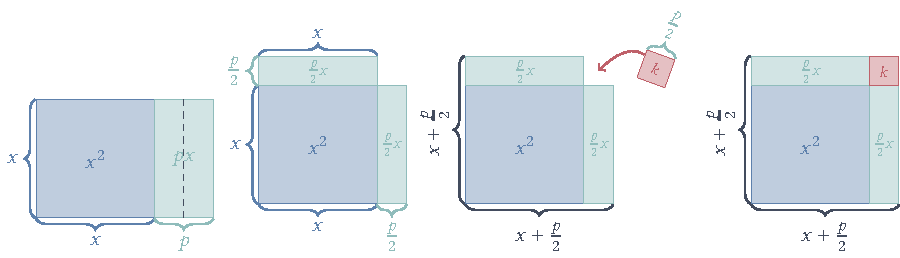
\includegraphics[width=0.9\textwidth]{imgs.tikz.058w}
		\end{center}
	\end{block}
\end{frame}
%   FRAME END   --==-=-=-=-=-=-=-=-=-=-=-=-=-=-=-=-=-=-=-=-=-=-=-=-=-=-=-=-=-=-=
%=-=-=-=-=-=-=-=-=-=-=-=-=-=-=-=-=-=-=-=-=-=-=-=-=-=-=-=-=-=-=-=-=-=-=-=-=-=-=-=


%=-=-=-=-=-=-=-=-=-=-=-=-=-=-=-=-=-=-=-=-=-=-=-=-=-=-=-=-=-=-=-=-=-=-=-=-=-=-=-=
%   FRAME START   -=-=-=-=-=-=-=-=-=-=-=-=-=-=-=-=-=-=-=-=-=-=-=-=-=-=-=-=-=-=-=
\begin{frame}[allowframebreaks, allowdisplaybreaks, t]{Example}{Expand \& Simplify}

	\prob Expand and simplify \( 2(x - 3)^2 - 3(x + 1)^2 \).

	\mref{oxfordIGCSEext5th-C02-S04-E11-Q24\cite{raynerCompleteMathematicsCambridge2018}\index{oxfordIGCSEext5th-C02!S04-E11-Q24}}

	\framebreak
	\soln \hfill
	\begin{align*}
		2(x - 3)^2 - 3(x + 1)^2 & = 2(x + \oneg  3)^2 + \oneg  3(x + 1)^2                                                                                              \\
		                        & = \cRed{2}\sqpar{(x + \oneg 3)(x + \oneg 3)} + \cDarkBlue{ \oneg 3}\sqpar{(x + 1)(x + 1)}                                            \\
		                        & = \cRed{2}\sqpar{x^2 + \oneg 6x + 9} + \cDarkBlue{ \oneg 3} \sqpar{x^2 + 2x + 1}                                                     \\
		                        & = \cRed{2}(x^2) + \cRed{2}( \oneg 6x) + \cRed{2}(9) + \cDarkBlue{ \oneg 3}(x^2) + \cDarkBlue{ \oneg 3}(2x) + \cDarkBlue{ \oneg 3}(1) \\
		                        & = 2x^2 + \oneg 12x + 18 + \oneg 3x^2 + \oneg 6x + \oneg 3                                                                            \\
		                        & = 2x^2 + \oneg 3x^2 + \oneg 12x + \oneg 3x + 18 + \oneg 3                                                                            \\
		                        & = \oneg 1x^2 + \oneg 18x + 15                                                                                                        \\
		                        & = \oneg x^2 - 18x + 15
	\end{align*}
\end{frame}
%   FRAME END   --==-=-=-=-=-=-=-=-=-=-=-=-=-=-=-=-=-=-=-=-=-=-=-=-=-=-=-=-=-=-=
%=-=-=-=-=-=-=-=-=-=-=-=-=-=-=-=-=-=-=-=-=-=-=-=-=-=-=-=-=-=-=-=-=-=-=-=-=-=-=-=

%=-=-=-=-=-=-=-=-=-=-=-=-=-=-=-=-=-=-=-=-=-=-=-=-=-=-=-=-=-=-=-=-=-=-=-=-=-=-=-=
%   FRAME START   -=-=-=-=-=-=-=-=-=-=-=-=-=-=-=-=-=-=-=-=-=-=-=-=-=-=-=-=-=-=-=
\begin{frame}[allowframebreaks, allowdisplaybreaks, t]{Example}{Completing The Square}

	\prob Solve the equation \( x^2 + 2x - 3 = 0 \) by completing the square.

	\mref{ma2c-5000-2022-Q2119a\cite{alfredssonMatematik5000Kurs2021}\index{ma2c-5000-2022-2000!Q2119a}}

	\framebreak
	\soln \hfill\\
	\begin{minipage}[t]{0.5\textwidth}
		\vspace{0pt}
		\begin{align*}
			x^2 + 2x - 3                                   & = 0 \\
			x^2 + 2x + \oneg 3                             & = 0 \\
			x^2 + 2x + \cRed{k} + \cRed{\oneg k} + \oneg 3 & = 0
		\end{align*}
	\end{minipage}
	\hspace{0.05\textwidth}
	\begin{minipage}[t]{0.4\textwidth}
		\vspace{0pt}
		\begin{center}
			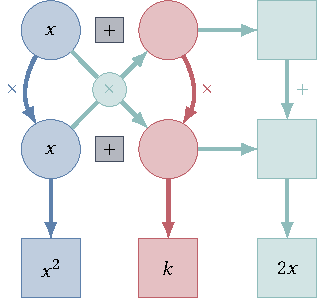
\includegraphics[width=0.8\textwidth]{imgs.tikz.057w}
		\end{center}
	\end{minipage}
	\hfill

	\framebreak

	\hfill\\
	\begin{minipage}[t]{0.5\textwidth}
		\vspace{0pt}
		\begin{align*}
			x^2 + 2x + \cRed{k} + \cRed{\oneg k} + \oneg 3 & = 0        \\
			x^2 + 2x + \cRed{1} + \cRed{\oneg 1} + \oneg 3 & = 0        \\
			(x + 1)^2 + \oneg 4                            & = 0        \\
			(x + 1)^2                                      & = 4        \\
			\sqrt{(x + 1)^2}                               & = \sqrt{4} \\
			\abs{x + 1}                                    & = 2
		\end{align*}
		Now we can consider both cases of \( \abs{x + 1} \).
	\end{minipage}
	\hspace{0.05\textwidth}
	\begin{minipage}[t]{0.4\textwidth}
		\vspace{0pt}
		\begin{center}
			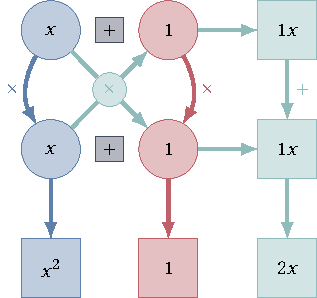
\includegraphics[width=0.8\textwidth]{imgs.tikz.057x}
		\end{center}
	\end{minipage}
	\hfill

	\framebreak

	\hfill\\
	\begin{minipage}[t]{0.45\textwidth}
		\vspace{0pt}
		\textbf{Case I: Positive Case}
		\begin{align*}
			x + 1 & = 2           \\
			x     & = \oneg 1 + 2 \\
			      & = 1
		\end{align*}
	\end{minipage}
	\hspace{0.05\textwidth}
	\begin{minipage}[t]{0.45\textwidth}
		\vspace{0pt}
		\textbf{Case II: Negative Case}
		\begin{align*}
			-(x + 1) & = 2                 \\
			x + 1    & = \oneg 2           \\
			x        & = \oneg 1 + \oneg 2 \\
			         & = \oneg 3
		\end{align*}

	\end{minipage}
	\hfill
\end{frame}
%   FRAME END   --==-=-=-=-=-=-=-=-=-=-=-=-=-=-=-=-=-=-=-=-=-=-=-=-=-=-=-=-=-=-=
%=-=-=-=-=-=-=-=-=-=-=-=-=-=-=-=-=-=-=-=-=-=-=-=-=-=-=-=-=-=-=-=-=-=-=-=-=-=-=-=


%=-=-=-=-=-=-=-=-=-=-=-=-=-=-=-=-=-=-=-=-=-=-=-=-=-=-=-=-=-=-=-=-=-=-=-=-=-=-=-=
%   FRAME START   -=-=-=-=-=-=-=-=-=-=-=-=-=-=-=-=-=-=-=-=-=-=-=-=-=-=-=-=-=-=-=
\begin{frame}[c]{Probability}{Dice and Coins}
	\hfill\\
	\begin{minipage}[t]{0.45\textwidth}
		\vspace{0pt}
		\textbf{Dice}
		\begin{itemize}
			\item \gdicei, \gdiceii, \gdiceiii, \gdiceiv, \gdicev, \gdicevi
			\item \bdicei, \bdiceii, \bdiceiii, \bdiceiv, \bdicev, \bdicevi
			\item \abdicei, \abdiceii, \abdiceiii, \abdiceiv, \abdicev, \abdicevi
			\item \rdicei, \rdiceii, \rdiceiii, \rdiceiv, \rdicev, \rdicevi
		\end{itemize}
		\textbf{Coins}
		\begin{itemize}
			\item \gcheads, \gctails
			\item \bcheads, \bctails
			\item \abcheads, \abctails
			\item \rcheads, \rctails
		\end{itemize}
	\end{minipage}
	\hspace{0.05\textwidth}
	\begin{minipage}[t]{0.45\textwidth}
		\vspace{0pt}
		\begin{exampleblock}{Sample Space Set Example}
			\begin{center}
				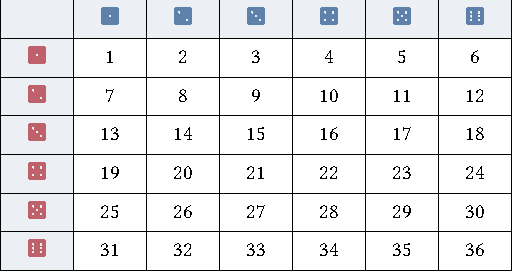
\includegraphics[width=0.9\textwidth]{imgs.tikz.05c9}
			\end{center}
		\end{exampleblock}
	\end{minipage}
	\hfill


\end{frame}
%   FRAME END   --==-=-=-=-=-=-=-=-=-=-=-=-=-=-=-=-=-=-=-=-=-=-=-=-=-=-=-=-=-=-=
%=-=-=-=-=-=-=-=-=-=-=-=-=-=-=-=-=-=-=-=-=-=-=-=-=-=-=-=-=-=-=-=-=-=-=-=-=-=-=-=

%=-=-=-=-=-=-=-=-=-=-=-=-=-=-=-=-=-=-=-=-=-=-=-=-=-=-=-=-=-=-=-=-=-=-=-=-=-=-=-=
%   FRAME START   -=-=-=-=-=-=-=-=-=-=-=-=-=-=-=-=-=-=-=-=-=-=-=-=-=-=-=-=-=-=-=
\begin{frame}[fragile]{Sets}{Well-Known}
	\hfill\\
	\begin{minipage}[t]{0.3\textwidth}
		\vspace{0pt}
		\begin{itemize}
			\item \(\cAquaBlue{ \set{} } \): \verb!\set{}!
			\item \(\cAquaBlue{ \suchthat } \): \verb!\suchthat!
			\item \(\cAquaBlue{ \setU } \): \verb!\setU!
			\item \(\cAquaBlue{ \setS } \): \verb!\setS!
			\item \(\cAquaBlue{ \setComp } \): \verb!\setComp!
			\item \(\cAquaBlue{ \setN } \): \verb!\setN!
			\item \(\cAquaBlue{ \setNs } \): \verb!\setNs!
			\item \(\cAquaBlue{ \setNi{\ge 4} } \): \verb!\setNi{\ge 4}!
			\item \(\cAquaBlue{ \setW } \): \verb!\setW!
		\end{itemize}
	\end{minipage}
	\begin{minipage}[t]{0.3\textwidth}
		\vspace{0pt}
		\begin{itemize}
			\item \(\cAquaBlue{ \setZ } \): \verb!\setZ!
			\item \(\cAquaBlue{ \setZp } \): \verb!\setZp!
			\item \(\cAquaBlue{ \setZn } \): \verb!\setZn!
			\item \(\cAquaBlue{ \setZs } \): \verb!\setZs!
			\item \(\cAquaBlue{ \setZi{\ge 4} } \): \verb!\setZi{\ge 4}!
			\item \(\cAquaBlue{ \setO } \): \verb!\setO!
			\item \(\cAquaBlue{ \setE } \): \verb!\setE!
			\item \(\cAquaBlue{ \setP } \): \verb!\setP!
			\item \(\cAquaBlue{ \setSquares } \): \verb!\setSquare!
			\item \(\cAquaBlue{ \setCubes } \): \verb!\setCubes!
		\end{itemize}
	\end{minipage}
	\begin{minipage}[t]{0.3\textwidth}
		\vspace{0pt}
		\begin{itemize}
			\item \(\cAquaBlue{ \setQ } \): \verb!\setQ!
			\item \(\cAquaBlue{ \setQp } \): \verb!\setQp!
			\item \(\cAquaBlue{ \setQn } \): \verb!\setQn!
			\item \(\cAquaBlue{ \setQs } \): \verb!\setQs!
			\item \(\cAquaBlue{ \setQi{\ge 4} } \): \verb!\setQi{\ge 4}!
			\item \(\cAquaBlue{ \setR } \): \verb!\setR!
			\item \(\cAquaBlue{ \setRp } \): \verb!\setRp!
			\item \(\cAquaBlue{ \setRn } \): \verb!\setRn!
			\item \(\cAquaBlue{ \setRs } \): \verb!\setRs!
			\item \(\cAquaBlue{ \setRi{\ge 4} } \): \verb!\setQi{\ge 4}!
			\item \(\cAquaBlue{ \setC } \): \verb!\setR!
		\end{itemize}
	\end{minipage}
	\hfill

\end{frame}
%   FRAME END   --==-=-=-=-=-=-=-=-=-=-=-=-=-=-=-=-=-=-=-=-=-=-=-=-=-=-=-=-=-=-=
%=-=-=-=-=-=-=-=-=-=-=-=-=-=-=-=-=-=-=-=-=-=-=-=-=-=-=-=-=-=-=-=-=-=-=-=-=-=-=-=

%=-=-=-=-=-=-=-=-=-=-=-=-=-=-=-=-=-=-=-=-=-=-=-=-=-=-=-=-=-=-=-=-=-=-=-=-=-=-=-=
% SECTION 
%=-=-=-=-=-=-=-=-=-=-=-=-=-=-=-=-=-=-=-=-=-=-=-=-=-=-=-=-=-=-=-=-=-=-=-=-=-=-=-=
\section{References}

\begin{frame}[allowframebreaks]{References}
	\printbibliography[title={References}]%
\end{frame}


\end{document}
%=+=+=+=+=+=+=+=+=+=+=+=+=+=+=+=+=+=+=+=+=+=+=+=+=+=+=+=+=+=+=+=+=+=+=+=+=+=+=+=
% END OF FILE
%=+=+=+=+=+=+=+=+=+=+=+=+=+=+=+=+=+=+=+=+=+=+=+=+=+=+=+=+=+=+=+=+=+=+=+=+=+=+=+=
